\documentclass[../AnalysisNoteJBuxton.tex]{subfiles}
\begin{document}

\subsubsection{\texorpdfstring{$\Lambda$}{TEXT} Reconstruction}
\label{LambdaReconstruction}

The following cuts were used to select good $\Lambda$ ($\bar{\Lambda}$) candidates:

\begin{enumerate}
 \item{Cuts Common to Both Daughters}
 \begin{enumerate}
  \item $|\eta| < 0.8$
  \item SetTPCnclsDaughters(80)
  \item SetStatusDaughters(AliESDtrack::kTPCrefic)
  \item SetMaxDcaV0Daughters(0.4)
 \end{enumerate}


 \item Pion Specific Daughter Cuts
 \begin{enumerate}
  \item $p_{T} > 0.16$
  \item DCA to prim vertex $>$ 0.3
 \end{enumerate} 
 
 \item Proton Specific Daughter Cuts
  \begin{enumerate}
  \item $p_{T} > $
  \begin{itemize}
   \item 0.5 ($p$)
   \item 0.3 ($\bar{p}$)
  \end{itemize}
   \item DCA to prim vertex $>$ 0.1 
 \end{enumerate} 
 
 \item Lambda Cuts
 \begin{enumerate}
  \item $|\eta| < 0.8$
  \item $p_{T} > 0.4$
  \item $|m_{inv} - m_{PDG}| <$ 3.8 MeV
  \item Cosine of pointing angle $>$ 0.9993
  \item OnFlyStatus = false
  \item Decay Length $<$ 60 cm
 \end{enumerate}  
 
\end{enumerate}


\begin{figure}[h]
\begin{minipage}{18pc}
\includegraphics[width=18pc]{3_DataSelection/Figures/MassAssHypotheses/canMassAssK0HypCompare_LamK0_wNoMisID.pdf}
\end{minipage}\hspace{2pc}
\begin{minipage}{18pc}
\includegraphics[width=18pc]{3_DataSelection/Figures/MassAssHypotheses/canMassAssK0HypCompare_ALamK0_wNoMisID.pdf}
\end{minipage} 
\caption[K$^{0}_{S}$ contamination in $\Lambda$($\bar{\Lambda}$) collection]{Mass assuming K$^{0}_{S}$-hypothesis for V0 candidates passing all $\Lambda$ ($\bar{\Lambda}$) cuts, i.e. assume the daughters are $\pi^{+}\pi^{-}$ instead of $p^{+}\pi^{-}$ ($\pi^{+}\bar{p}^{-}$).  The slight peak around $m_{inv}$ = 0.5 GeV/c$^{2}$ likely contains misidentified K$^{0}_{S}$ particles in our $\Lambda$ collection.  If one simply cuts out the entire peak, good $\Lambda$ particles will be lost.  Ideally, the $\Lambda$ selection and K$^{0}_{S}$ misidentification cuts are selected such that the peak is removed from this plot while leaving the distribution continuous.}
  \label{fig:MassAssK0ShortHyp_cLamK0}
\end{figure}

\begin{figure}[h]
  \centering
  \includegraphics[width=100mm]{3_DataSelection/Figures/MassAssHypotheses/canMassAssK0HypCompare_LamK0_wNoMisID.pdf}
  \caption[K$^{0}_{S}$ contamination in $\Lambda$ collection]{Mass assuming K$^{0}_{S}$-hypothesis for V0 candidates passing all $\Lambda$ cuts, i.e. assume the daughters are $\pi^{+}\pi^{-}$ instead of $p^{+}\pi^{-}$.  The slight peak around $m_{inv}$ = 0.5 GeV/c$^{2}$ likely contains misidentified K$^{0}_{S}$ particles in our $\Lambda$ collection.  If one simply cuts out the entire peak, good $\Lambda$ particles will be lost.  Ideally, the $\Lambda$ selection and K$^{0}_{S}$ misidentification cuts are selected such that the peak is removed from this plot while leaving the distribution continuous.}
  \label{fig:MassAssK0ShortHyp_LamK0}
\end{figure}

\begin{figure}[h]
  \centering
  \includegraphics[width=100mm]{3_DataSelection/Figures/MassAssHypotheses/canMassAssK0HypCompare_ALamK0_wNoMisID.pdf}
  \caption[K$^{0}_{S}$ contamination in $\bar{\Lambda}$ collection]{Mass assuming K$^{0}_{S}$-hypothesis for V0 candidates passing all $\bar{\Lambda}$ cuts, i.e. assume the daughters are $\pi^{+}\pi^{-}$ instead of $\pi^{+}\bar{p}^{-}$.  Similar to Figure \ref{fig:MassAssK0ShortHyp_LamK0}}
  \label{fig:MassAssK0ShortHyp_ALamK0}
\end{figure}

\begin{figure}[h]
  \centering
  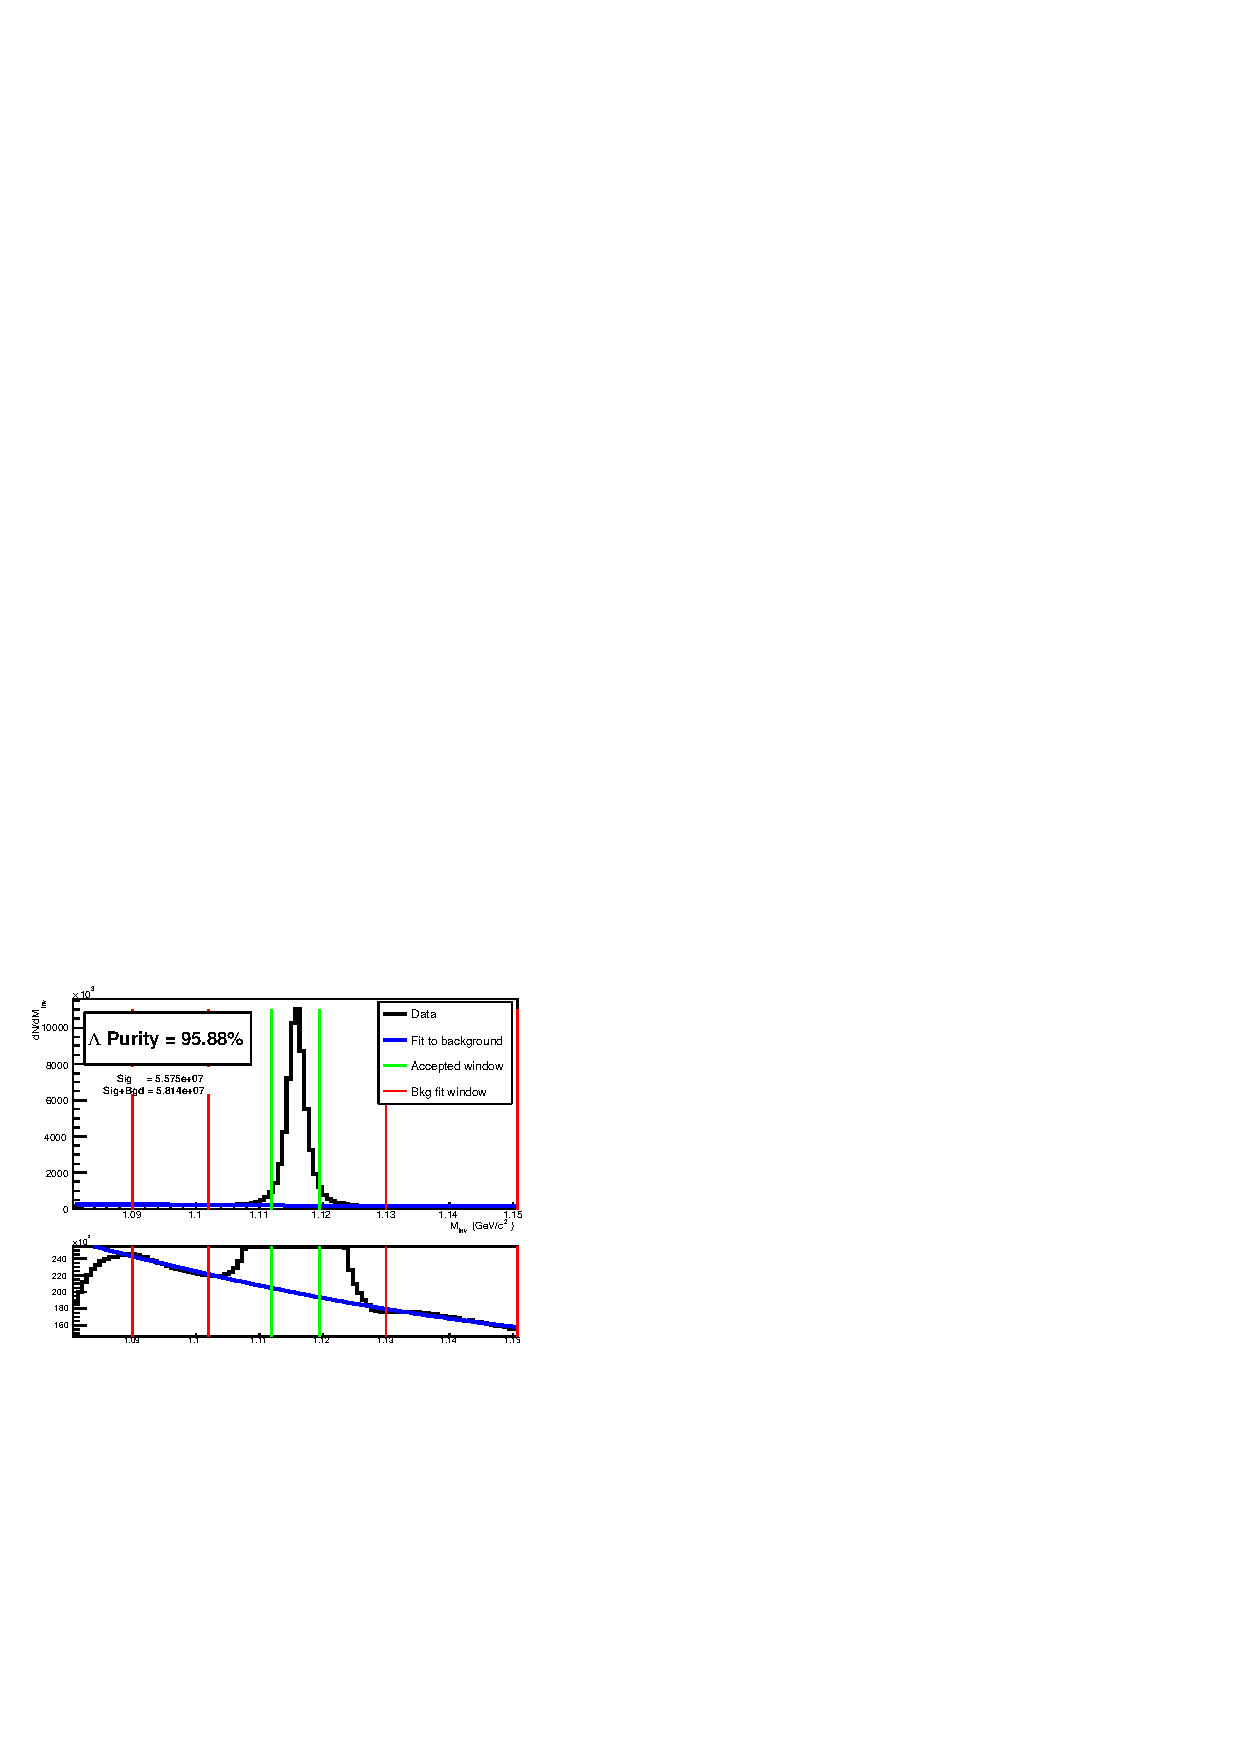
\includegraphics[width=100mm]{3_DataSelection/Figures/LamPurity_LamK0.pdf}
  \caption[$\Lambda$ Purity]{$\Lambda$ Purity}
  \label{fig:LamPurity}
\end{figure}

\end{document}